\section{Modelliersprache}
Zur Beschreibung wurde, entgegen der in dem Projekt genannten Sprache, MyHDL\footnote{\url{http://myhdl.org}} genutzt. Es wurde uns von einem Kommilitonen nahe gelegt \textit{nicht} VHDL zu nutzen, da dies einen Großteil der Zeit in Anspruch nimmt die Sprache zu lernen. Diese Zeit würde später fehlen, wenn man den Mikrocontroller implementieren möchte
MyHDL ist ein Python-Modul, welches dazu genutzt wird Python als Hardwarebeschreibungssprache zu nutzen. Außerdem können damit auch Tests geschrieben werden, die zur Verifikation der Devices dient.
Ein Beispiel ist zu finden unter \autoref{HW:DFlipFop}.

\begin{figure}[h]
\small
\begin{pythoncode}
from myhdl import *
 
def dff(q, d, clk):
 
    @always(clk.posedge)
    def logic():
        q.next = d
 
    return logic
\end{pythoncode}
\caption{\label{HW:DFlipFop}D-FlipFlop}
\end{figure}

In Zeile drei werden sämtliche Ports der Komponente deklariert. Dabei werden -- im Gegensatz zu VHDL -- keine Spezifikationen wie input/output oder Bitlänge definiert. Diese werden laut Konvention nur in dem Kommentar der ``Funktion'' definiert.\\
Der Dekorator\footnote{\url{https://wiki.python.org/moin/PythonDecorators}} in Zeile 5 wird benutzt um zu spezifizieren, wann die dekorierte Funktion ausgeführt werden soll. In diesem Falle wird gesagt, dass bei einer steigenden Flanke des clk-Ports die Funktion ausgeführt werden soll.\\
Die eigentliche Logik der Komponente befindet sich in Zeile 7. Hier wird gesagt, dass im nächsten Augenblick der Wert von \textit{q d} sein soll.
In Zeile 9 wird die dekorierte Funktion zurückgegeben, d.h. sie wird in der Simulation und Transformation berücksichtigt.\\
Gut zu sehen sind an diesem Beispiel die Vor- und Nachteile von Python als Hardwarebeschreibungssprache. Ein Nachteil ist, dass man die genaue Spezifikation eines Ports nicht direkt angeben kann, z.B. deren Bitweite oder Typ. Dies kann zu Fehlern führen und zu viel Frust. MyHDL entscheidet die Eigenschaften durch statische Analyse des Quellcodes.\\
Vorteile hingegen sind der große Umfang der Python-Bibliotheken, die man sehr gut zum Testen der Komponenten nutzen kann, z.B. reguläre Ausdrücke, Listen oder Hashmap, sowie die einfache Erlernbarkeit und viele Syntaktische Feinheiten.\\

\section{Design}
\begin{figure}
\vspace{-4em}
\centering
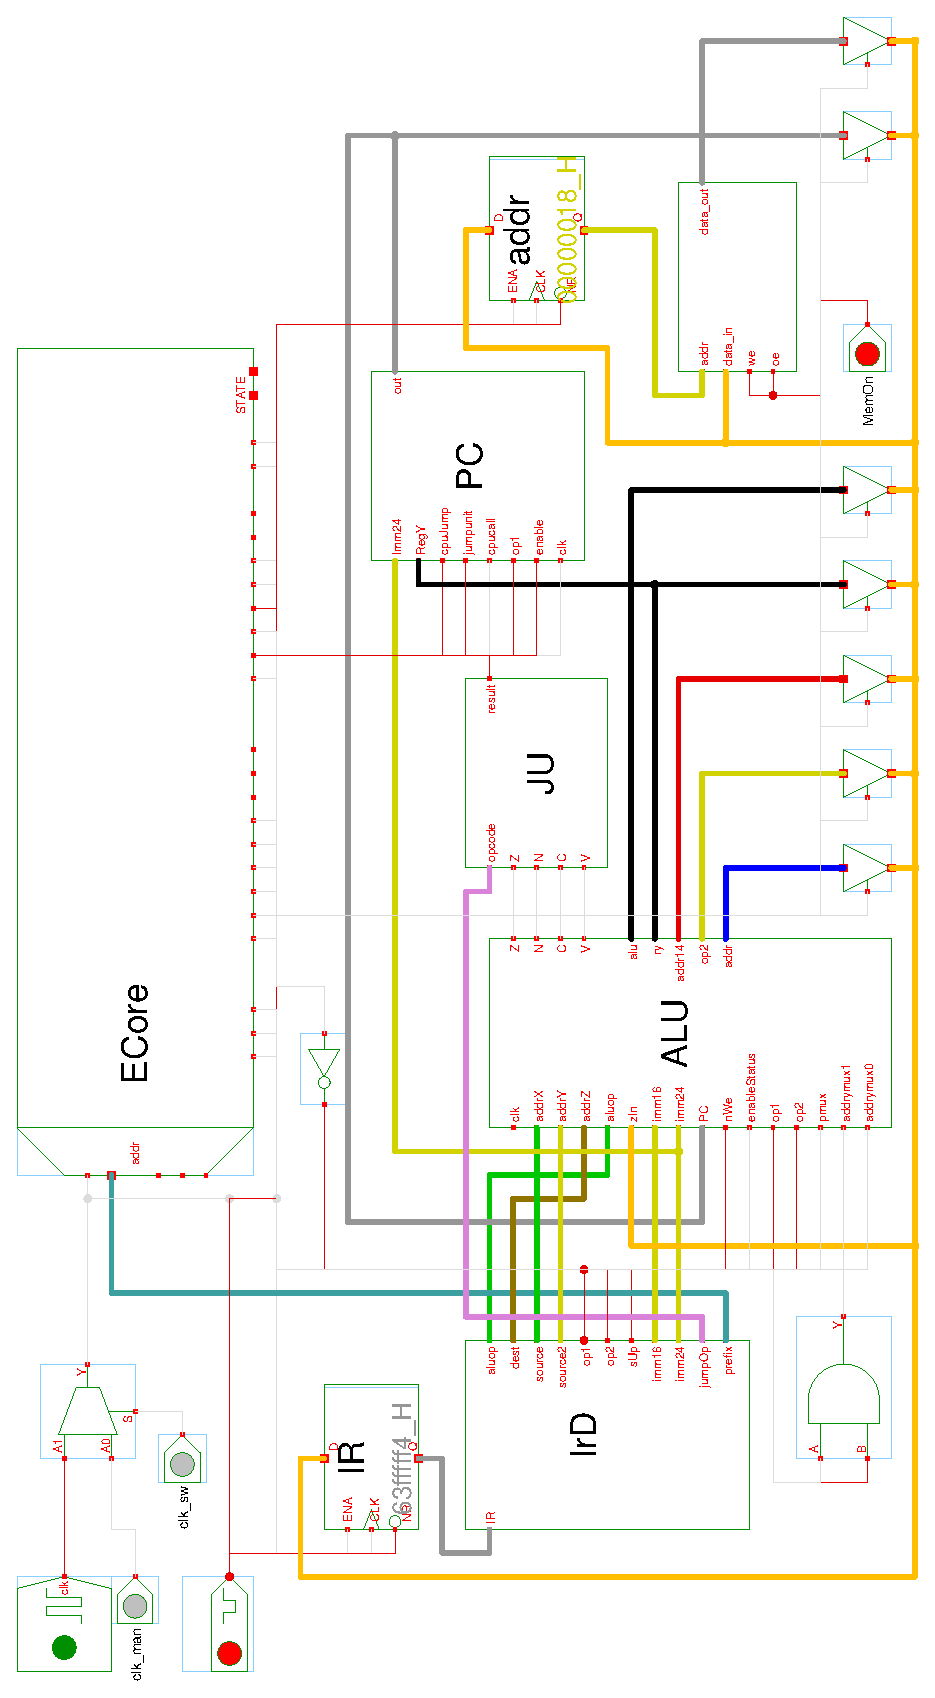
\includegraphics[width=.8\textwidth]{images/overview.eps}
\caption{\label{HW:Overview}Übersicht des MK}
\end{figure}
Das Design der Mikrocontrollers ist sehr stark am D-Core\footnote{\url{http://tams-www.informatik.uni-hamburg.de/applets/hades/webdemos/60-dcore/t3/processor.html}} orientiert, mit einem zentralen Bus, einem Steuerwerk, einer Abstraktion für den Speicher, sowie Elementen, die mit Hilfe des Busses miteinander kommunizieren. Wie man in der \autoref{HW:Overview} sehr gut sehen kann ist die Verbindung zwischen den einzelnen Komponenten auf ein Minimum gehalten. Einzige Ausnahme bildet hierbei der Instruction-Decoder. Auf die einzelnen Komponenten wird in den Folgenden Abschnitten noch genauer eingegangen.\\
Die Entscheidung zu dieser Anordnung kam aus der Überlegung heraus, dass wir uns an etwas bestehendem orientieren wollten. Deswegen ist verfügt er über einen Bus und verschiedene TriState-Dioden, die von einer Zentralen Einheit angesteuert werden, in unserem Fall das Steuerwerk oder CPU genannt. Doch genau hier liegt auch das Problem, denn die CPU ist nicht in der Lage aktiv werte an Komponenten zu senden, sondern schaltet nur Leitungen an oder aus. Auf dieses Problem wird später in der ALU auch noch genauer eingegangen. So gibt es an einigen Stellen für bestimmte Probleme maßgeschneiderte Lösungen.\\
Ein dennoch großer Vorteil eines gemeinsamen Busses ist die einfache Erweiterbarkeit des Systems. So hatten wir am Anfang gar nicht mit einer RS232-Schnittstelle gerechnet, konnte diese später jedoch Problemlos einfügen, indem sie am Bus lauscht/schreibt und von der CPU geschaltet wird.\\
Die eigentliche Beschreibung des Mikrocontrollers erfolgt letztendlich in Python und kann im Beigelegten Projektordner eingesehen werden.

\subsection{Steuerwerk}
Unser Steuerwerk (CPU) ist eine State-Maschine (\ref{HW:CPU-State}), die anhand eines Präfix in den nächsten Status gelangt. In einem Status ist genau festgehalten zu welchem Zeitpunkt welche Steuerleitung (de-)aktiviert wird. Hier ist es möglich Substates zu haben (realsiert mit Hilfe eines hochlaufen Counters), falls dieser Befehl mehr als einen Takt benötigt um z.B. auf die Antwort der MMU zu warten. Das Bereit sein wird asynchron gemeldet, das heißt über eine eingehen Steuerleitung. 

\begin{figure}[h]
TODO: state chart machen
\begin{tikzpicture}[semithick]
    \tikzstyle{every state}=[fill=white,draw=none,text=black]
    \node[initial,state]    (F)                        {$Fetch$};
    \node[state]            (D)    [below of=F]        {$Decode$};
    
    \path[->] (F)     edge    node {}    (D);
\end{tikzpicture}
\caption{\label{HW:CPU-State}Cpu}
\end{figure}

\subsection{Instruction Decoder}
Der Instruction Decoder (IrD) ist zuständig dafür, einen 32Bit langen Wert in seine Einzelteile zu zerlegen und den einzelnen Komponenten zur Verfügung zu stellen. Dies soll ohne Takt geschehen, sondern sofort. Eine Entsprechende Abbildung ist unter \autoref{HW:IRD} zu sehen.\\
\begin{figure}[h]
\centering
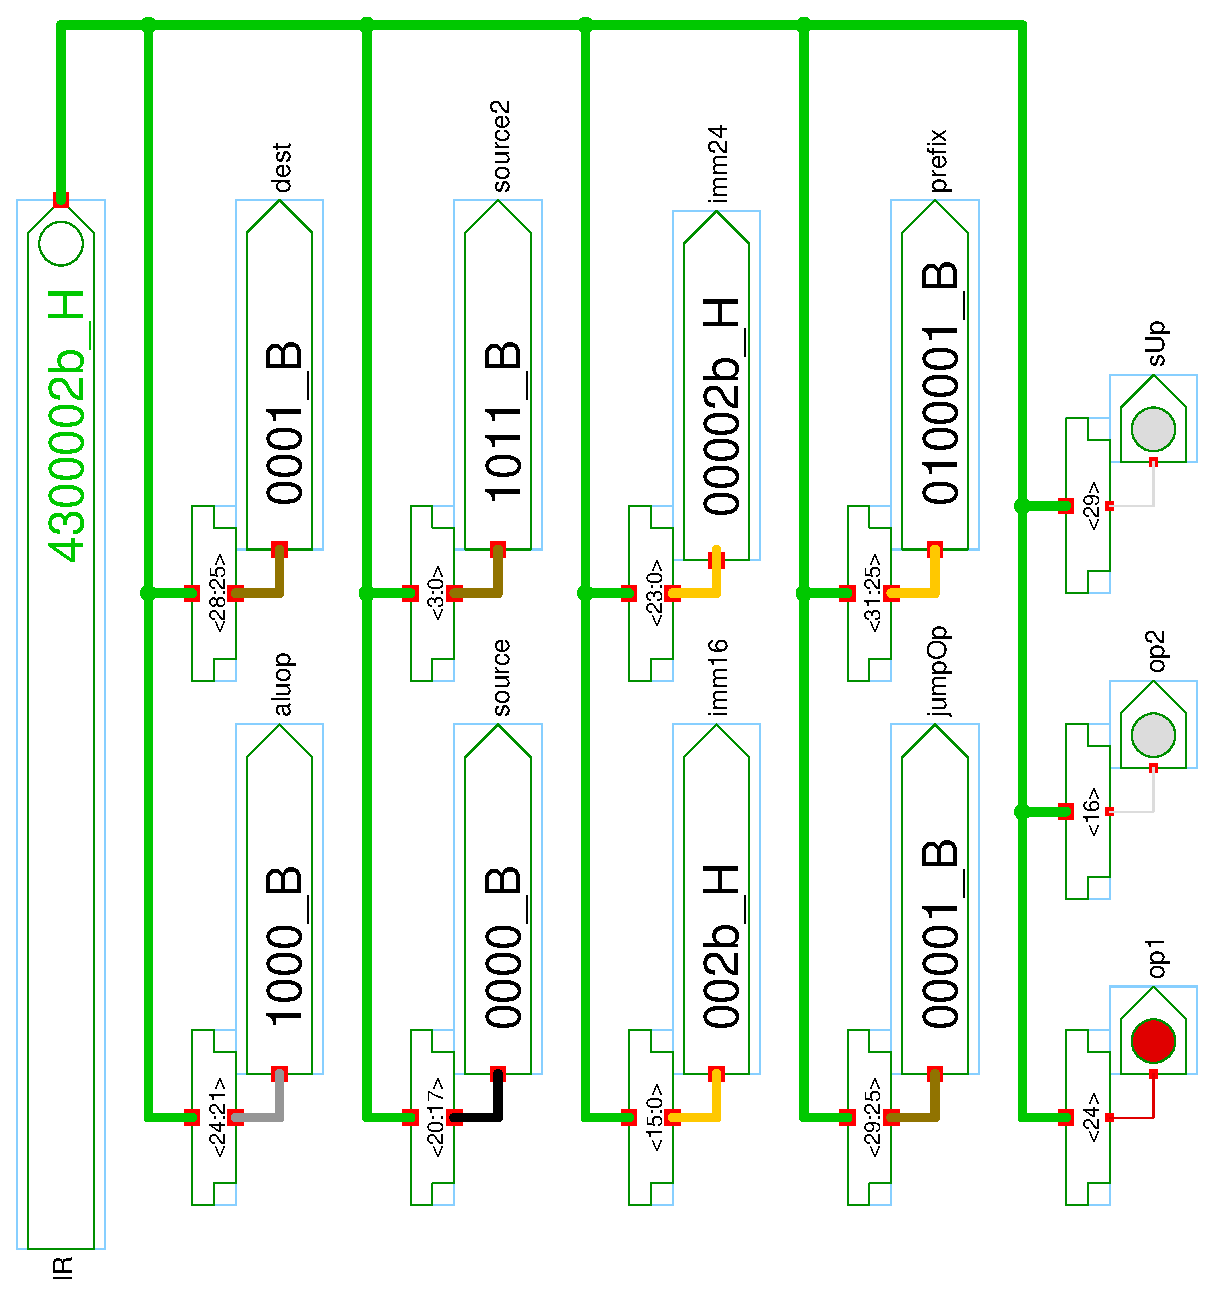
\includegraphics[width=.8\textwidth,angle=270]{images/ir.eps}
\caption{\label{HW:IRD}Instruction Decoder}
\end{figure}
Der IrD stellt 8 Werte und 3 Flags bereit. Die Einzelnen Werte stehen für:

\begin{itemize}
  \item aluop -- Der Op-code für die ALU
  \item dest --  Die Zieladresse für die Registerbank (Z)
  \item source -- Die Quelladresse für die Registerbank (X)
  \item source2 -- Die zweite Quelladresse für die Registerbank (Y)
  \item imm16 -- Ein 16Bit breiter Immediate Wert für Berechnungen
  \item imm24 -- Ein 24Bit breiter Immediate Wert für Berechnungen
  \item jumpop -- Der Op-code für die Sprungeinheit.
  \item prefix -- Das Instruktionsprefix für die CPU
\end{itemize}
Mit Hilfe der einzelnen Werte und Flags ist es nun möglich einen Befehl gemäß unserer Befehlsstruktur auszuführen. Da Werte nicht immer sinnig sein müssen, z.B. bei einem Sprungbefehl kann ein unsinniger Aluop entstehen, ist für die Hardware nicht weiter schlimm. Denn die berechnet einfach, wird ihr Ergebnis aber nie auf den Bus schreiben, denn die CPU unterbindet dies.
\subsection{ALU}
\begin{figure}[hbt]
\centering
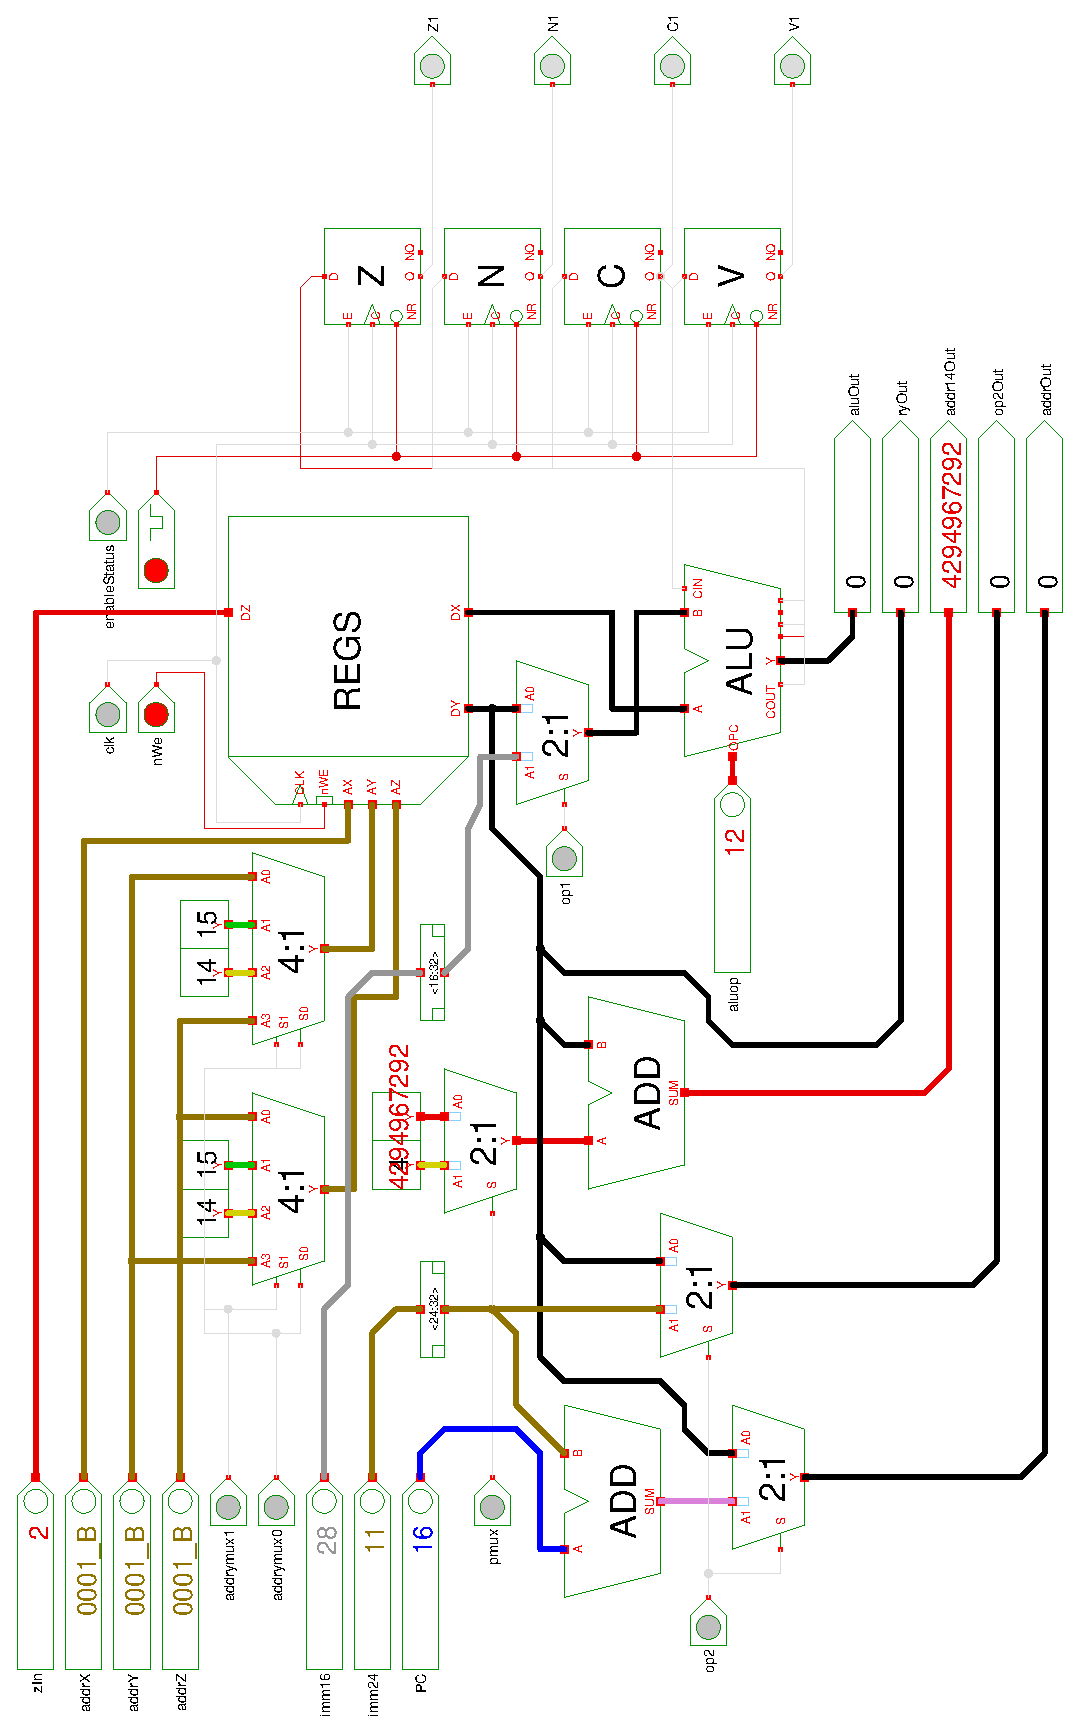
\includegraphics[width=.8\textwidth]{images/alu.eps}
\caption{\label{HW:ALU}Address, Arithmetisch und Logische Einheit}
\end{figure}
Die ALU dient in unserem Mikrocontroller nicht allein zur Berechnung von Ergebnissen, sondern sie ist ein Sammelbegriff für alle Arten von mathematischen Operationen, wie z.B. Adress- oder Stackoffsetberechnung.\\
Die Registerbank hat 16 Slots, wobei einigen Plätzen besondere Eigenschaften und Bedeutungen zugewiesen wird. Dies hat nichts mit der ABI der Programme zu tun, sondern ist in der Hardware festgelegt und verdrahtet.
\begin{itemize}
  \item[0 --] Diese Adresse ist immer 0 und kann sowohl gelesen als auch beschrieben werden. Der Wert ändert sich nie
  \item[14 --] Die ist der Stackpointer. Wann immer eine Push/Pop Operation ausgeführt wird, wird das 14te Register mit Hilfe der Hardware angepasst.
  \item[15 --] Die Rücksprungadresse. Mit Hilfe des Call-Befehl wird der aktuelle Programmcounter in das Regsiter 15 abgelegt.
\end{itemize}
\subsection{Jumpunit}
\begin{figure}[h]
\centering
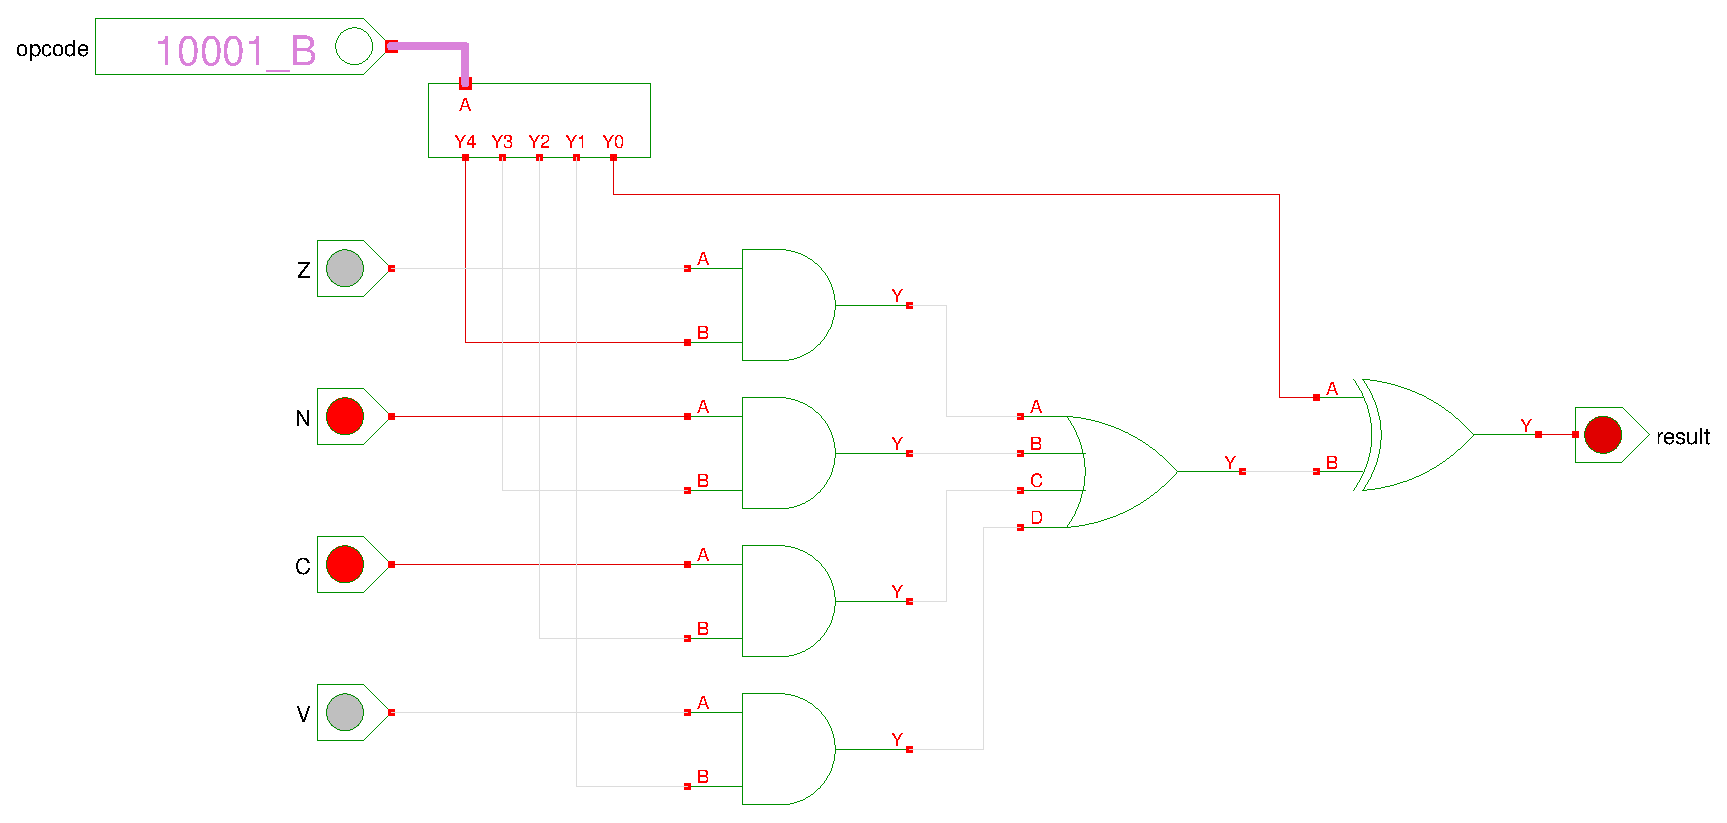
\includegraphics[width=1\textwidth]{images/ju.eps}
\caption{\label{HW:JU}Sprung-Einheit}
\end{figure}
\subsection{Programmcounter}
\begin{figure}[h]
\centering
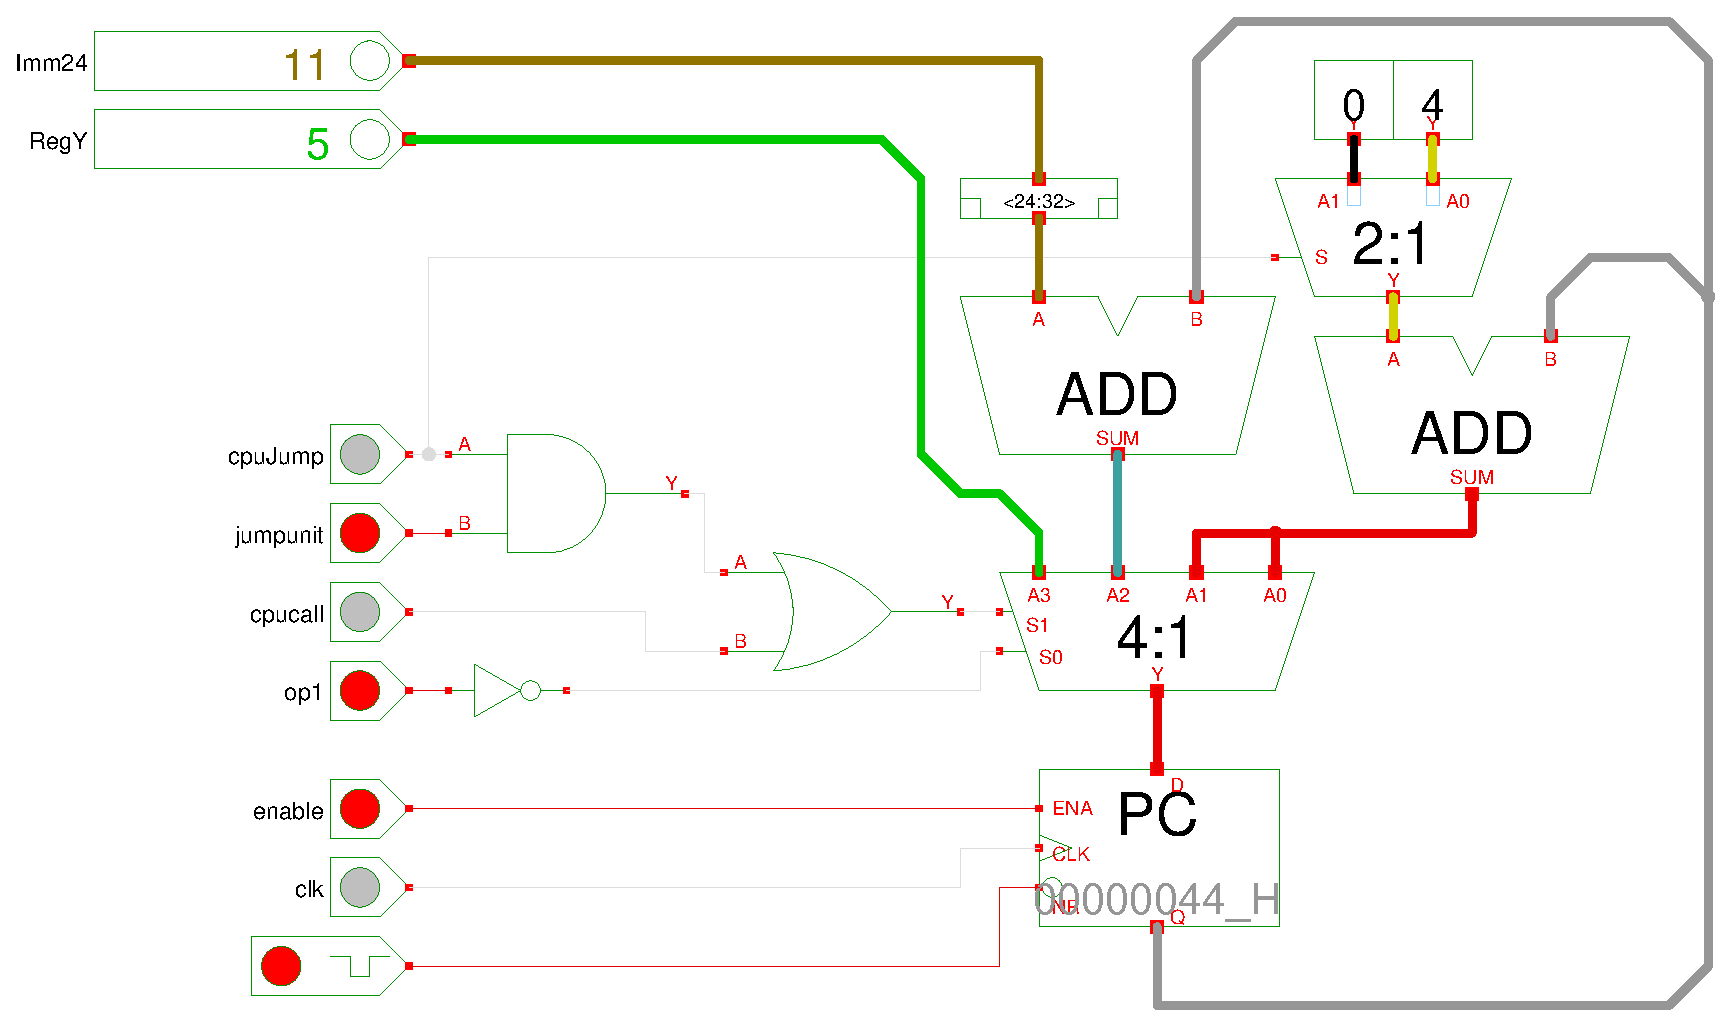
\includegraphics[width=1\textwidth]{images/pc.eps}
\caption{\label{HW:PC}Programmcounter}
\end{figure}
\subsection{Memory}
